\subsection{Product perspective}
Our product is an ecosystem of applications designed from scratch to accomplish different purposes.

In particular, the system is designed to be a set of three subsystems interacting with each other, as shown in the following diagram:

\FloatBarrier
\begin{figure}[!ht]
	\centering
	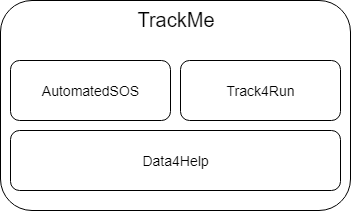
\includegraphics[scale = 0.70]{Images/general_structure.png}\\[1.0 cm]
	\caption{TrackMe ecosystem}
\end{figure}
\FloatBarrier

Data4Help is the underlying backbone of our system that collects data from end users and makes it available to the third party applications. 

The other two subsystems are built on top of Data4Help and provide to the users different services: AutomatedSOS offers an automated way of calling an ambulance in case of emergency, while Track4Run gives to the end users a platform to organize and participate to run events.

The following subsections give a more detailed analysis of the domain of each subsystem and are accompanied with the corresponding class diagrams. The aim of these diagrams is to identify the main actors and components of the subsystems and the relationship between them.

\newpage

\subsubsection{Data4Help}
Data4Help is meant to be a stand-alone system that works as a gateway between user data \textit{producers} and the third parties, which are data \textit{consumers}. The central actor of this system is the user.

Each user can configure multiple data sources: each of them can collect different parameters that together form the user data. On the other hand, third parties can make some data requests, that can be targeted to a single user data or a group of data.

These requests can be of two different types: subscriptions, which will cause the third party to be updated whenever the chosen data set changes, or single requests.

Bearing these considerations in mind, the following diagram is given to better describe the domain of the application.

\FloatBarrier
\begin{figure}[h!]
	\centering
	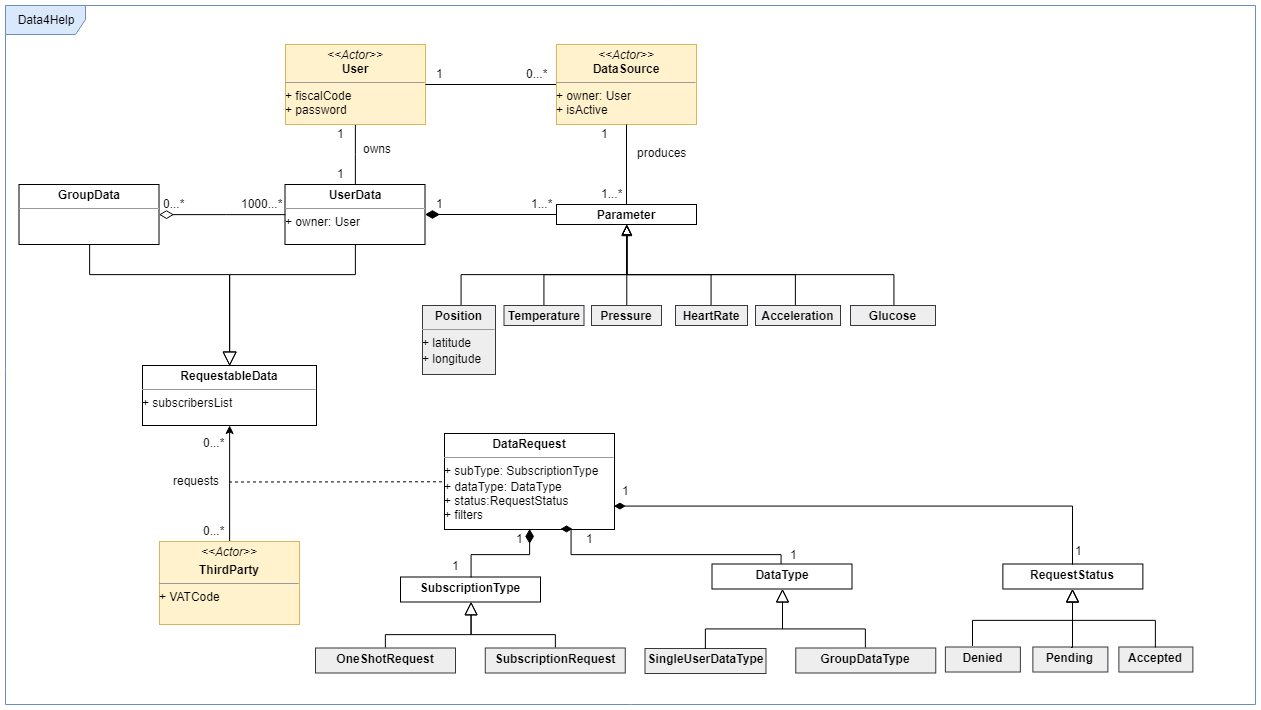
\includegraphics[width = \linewidth] {../Diagrams/ClassDiagram-General.png}\\[1.0 cm]
	\caption{Data4Help Class Diagram}
\end{figure}
\FloatBarrier

Please note that the parameter types listed here are the most commonly used in many kind of applications, but this doesn't exclude that more parameter types can be added in future.

\newpage

\subsubsection{AutomatedSOS}
Differently from the previous one, AutomatedSOS is an application which relies on other systems, such as an Ambulance Calling System and Data4Help, to provide a specific service to the customers. 
The offered service is a monitoring system for Data4Help users, in which some threshold values can be set for each vital parameter. If one of these parameters exceeds his thresholds, this will cause the system to send the GPS location of the user in danger to an ambulance.

In this perspective, the AutomatedSOS system can be seen as one of the third parties of the previous diagram: for each new user, it makes a subscription request for the data of that user to the Data4Help system

\FloatBarrier
\begin{figure}[h!]
	\centering
	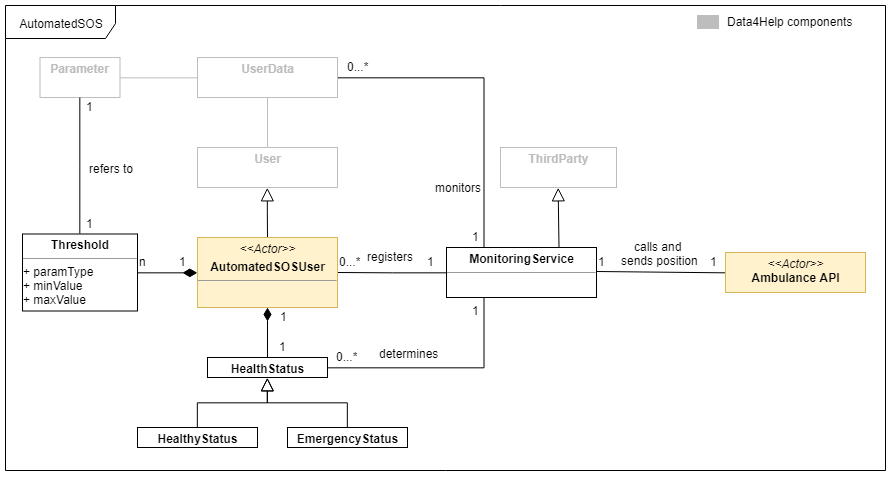
\includegraphics[width = \linewidth] {../Diagrams/ClassDiagram-AutomatedSOS.png}\\[1.0 cm]
	\caption{AutomatedSOS Class Diagram}
\end{figure}
\FloatBarrier

\newpage

\subsubsection{Track4Run}
Like AutomatedSOS, Track4Run is an application that uses Data4Help to monitor some of its users, in particular the runners who participate to run event.
These run events are created and managed by organizers. On the other hand, spectators can see the position of the runners by using the dedicated service.

\FloatBarrier
\begin{figure}[h!]
	\centering
	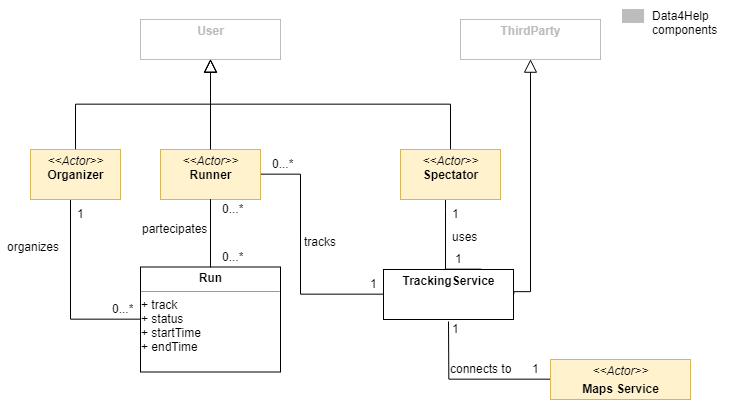
\includegraphics[width = \linewidth] {../Diagrams/ClassDiagram-Track4Run.png}\\[1.0 cm]
	\caption{Track4Run Class Diagram}
\end{figure}
\FloatBarrier

\newpage
	
\subsection{Product functions}
Considering all the goals this system has to accomplish, an additional and more detailed description is here provided for the main functions that each subsystem has to accomplish.

\subsubsection{Data4Help - User Data Acquisition}
Data acquisition is the focus of Data4Help and it is also fundamental for all the subsystems built on top of it.

In order to provide this feature, the system must give to the user the possibility to store his position and state of health and share them with the interested third parties.
 
This kind of data can be acquired from different data sources, such as external applications, smartphones, smartwatches or other similar devices. In order to collect the data from them, the user must firstly synchronize the device or application with Data4Help by providing his credentials and accepting the new data source.

The data source will then be able to retrieve real-time data from the user and send them to the Data4Help system, which in turn makes them available to the authorized third parties.

In any time the user must be able to add a new data source, decide which parameter can be monitored from which device, add a new data source or stop an existing one from sending new data.

\subsubsection{Data4Help - User Data Sharing}
The system gives the possibility to third parties to register to the service and request users' data.

Data requests can be done by using an API which will be provided in order to encourage third parties to develop their own applications integrated with Data4Help services.

There are two different types of requested data: single users' data or multiple users' data. The first ones are forwarded to the user and need to be explicitly accepted by him before being carried out. On the other hand, multiple users' data requests do not need user approval, but they can be completed only if the number of users satisfying the search filters are enough to guarantee a proper data anonymization.

In order to be continuously updated, third parties can also make data subscription requests. In this case, a callback interface must be provided in order to be notified as soon as the monitored data changes.

Also, in this case, the user can at any time decide to revoke to the third parties the permission to access his data.

\subsubsection{AutomatedSOS - Health Emergency Monitoring}
AutomatedSOS continuously monitors the health parameters selected by the user, exploiting the Data4Help system's data. The user of this system is provided with the possibility to set some thresholds, that can be default or changed at any moment.

As soon as one of them exceeds its pre-defined threshold, the system must contact an external interface that sends to an ambulance the position of the user in danger.

Between the emergency detection and the ambulance call, the user is notified that a threshold has been exceeded and a small window of time is granted to the user to abort the operation, so to minimize false-positive situations.

\subsubsection{Track4Run - Run Events Management}
Run events are the central focus of the Track4Run subsystem. Its main goal is to provide the users with the possibility of organizing, participating and watching runs.

Each user will have the possibility to see all the runs that he has created and to create a new one. Creating a run means deciding a date and hour for starting and ending and select a track from a map: for this, the access to an external service of map visualization like Google Maps will be necessary. This run can then be later deleted or postponed, or the track can be changed, and on each of these changes, the participant runners shall be informed.

The system also offers the possibility to search for ongoing runs and other planned runs that can be joined. In the first case, the user can decide a run to monitor and a map will appear with the live position of all the runners that are involved in that event. In the second case, joining a run means that somebody can track your position while you are running and you will receive notifications if some details change before it starts.

The position tracking is made using Data4Help, so the user's corresponding credentials are needed in order to use this application.

\subsection{User characteristics}

\subsubsection{Actors}
In the following section, a more specific characterization of the users and actors of each system is provided, based on the domain description that was previously offered.

\begin{itemize}
\item \textbf{Data4Help User}: in the Data4Help system the user is only a provider of information. After registration, he can access the platform's functionalities by logging in the system.
 
\item \textbf{Third Party}: any organization or software that wants to access the user's data. This is the main direct user of the Data4Help services. He can access the system by registering with a trusted authentication method and using the token generated by his registration. 
AutomatedSOS and Track4Run are considered to be third parties according to this definition, even if they don't belong to an external organization.

\item \textbf{Data Source}: any application or device that can be configured by the user to synchronize itself with the system, meaning that it can be authenticated using the user's Data4Help credentials.
We can imagine that the existing companies in the wearable and smart devices world can make a deal with TrackMe to enable the users of their systems to add a Data4Help account, therefore synchronizing the device/application. 

\item \textbf{AutomatedSOS User}: is imagined to be a Data4Help user who wants to carefully monitor his health status, such as an elder user or someone who is undergoing or recovering from an illness.

\item \textbf{Ambulance Calling System}: a supposedly existing external system that is able to provide an interface to access the national health-care system, used by AutomatedSOS.

\item \textbf{Run Organizer}: a user who creates a run event. He must be a Data4Help user who has downloaded the Track4Run application.
 
\item \textbf{Runner}: a user who participates to an organized run. Like the previous one, he has to be already registered to Data4Help in order to use the application.

\item \textbf{Run Spectator}: a Data4Help user that accesses the Track4Run application to follow an ongoing run event.

\item \textbf{Map Application}: an external service which provides a reliable visualization and tracking service of the GPS position on a map. An example could be \textit{Google Maps}. This must be accessed from the Track4Run application through some kind of interface.

\item \textbf{System Administrator}: someone who is in charge of administrating and maintaining the system. His credentials are generated by the application itself before the deployment, hence he doesn't have to register.
\end{itemize}

\subsection{Assumptions, dependencies and constraints}

\subsubsection{Domain Assumptions}
\begin{itemize}
    \item \textbf{[D1]} Fiscal code uniquely identifies a user of the system.
    \item \textbf{[D2]} Every user owns at least one device capable of retrieving correct real-time health parameters and location
    \item \textbf{[D3]} User devices must grant to the system access to the requested data
    \item \textbf{[D4]} User devices must be continuously connected to the internet
    \item \textbf{[D5]} VAT code uniquely identifies a third party in the system
    \item \textbf{[D6]} Third parties know the monitored user Fiscal Code
    \item \textbf{[D7]} Third parties are able to provide callback interfaces
    \item \textbf{[D8]} AutomatedSOS has access to parameters that can be useful for identifying an emergency status
    \item \textbf{[D9]} There exists an API through which AutomatedSOS can pass to an ambulance information about the identity, the location and the vital parameters of the person in trouble
    \item \textbf{[D10]} Track4Run athlete wears the monitoring device during the whole run
    \item \textbf{[D11]} There is a system providing an API to visualize GPS data on a map.
\end{itemize}

\subsubsection{Software dependencies}
The considered system relies on external software interfaces to accomplish the previously described functions and make the resulting product more lightweight.

\begin{itemize}
    \item \textbf{Ambulance Calling System}
\end{itemize}

AutomatedSOS must call an ambulance to rescue the user given his geographical position. For the sake of simplicity, we assume that the national health service offers to the external applications an API that automatically calls an ambulance and sends to it the coordinates to reach the mentioned location.

\begin{itemize}
    \item \textbf{City Maps}
\end{itemize}

Track4Run users need to use city maps to accomplish different tasks: organizers use them to create events and trace the path of the runs, athletes to check the information about the track in the created events and spectators to display the real-time positions of the athletes on the path during the run. An API of this kind could be Google Maps API, which gives accurate real-time information for mapping, navigation, and places.

\begin{itemize}
    \item \textbf{Mobile Operating System}
\end{itemize}

The two subsystems, AutomatedSOS and Track4Run, are mobile applications that run on some physical smart-devices. For this reason, they need an operating system to interface with such as Android or iOS.
\subsubsection{Hardware constraints}

\begin{itemize}
    \item \textbf{Servers}
\end{itemize}
Our system needs to store huge amounts of data coming from single users. For this reason, a strong underlying server architecture is needed to develop the back-end part of the system. Possibly the resulting architecture can take inspiration from the classic three-tier web application architecture composed of a web server, an application server, and a database server.

\begin{itemize}
    \item \textbf{Sensors and Smart Devices}
\end{itemize}
Data4Help acquires data from the previously defined data sources, which are devices such as smartwatches, smartphones, wearables and other. Hence, even if they are not directly part of the system, the reliability and availability of the system's data are strongly connected to the existence of reliable sensors and devices that can collect and send data from them in real-time.

\begin{itemize}
    \item \textbf{GPS}
\end{itemize}
As concerns the geographical position of the users, Data4Help should give it to the subscribed third parties, if requested. Moreover, AutomatedSOS must know it to send correct info to the ambulances and Track4Run use the user's geographical position to display it on the run path to the spectators during the run. For this reason, in order to retrieve the correct value for the geographical position of the user, this last should have at least one active device with GPS enabled.

\begin{itemize}
	\item \textbf{2G/3G/4G internet connection}
\end{itemize}
Even if the user is not connected via WiFi or Ethernet cable to the internet, our system (in particular AutomatedSOS and Track4Run) has to retrieve user's data in spite of the user's current position. For this reason, the system relies on 3G / 4G technology to grant to the user a non-stop internet access.